\section*{Scoring}
%At the end of the final round, each player scores some number of points determined by the treasures they have collected throughout the game.

\begin{minipage}{1.5cm}
\tikz{\node[draw, thick, minimum width=1.5cm, minimum height=1.5cm, inner sep=0pt, rounded corners=3mm] at (0,0) {
\includegraphics[width=1.0cm]{Images/gold-coins-large.png}};}
\end{minipage}
\ 
\begin{minipage}{6cm}
\raggedright
\goldtext
\end{minipage}

\begin{minipage}{1.5cm}
\tikz{\node[draw, thick, minimum width=1.5cm, minimum height=1.5cm, inner sep=0pt, rounded corners=3mm] at (0,0) {
\includegraphics[height=1.25cm]{Images/bottle-of-rum2.png}};}
\end{minipage}
\ 
\begin{minipage}{6cm}
\raggedright
Score a number of points based on how many bottles of rum you have at the end of the game, 0:0, 1:1, 2:4, 3:9, 4+:0.
\end{minipage}

\begin{minipage}{1.5cm}
\tikz{\node[draw, thick, minimum width=1.5cm, minimum height=1.5cm, inner sep=0pt, rounded corners=3mm] at (0,0) {
\includegraphics[width=1.0cm]{Images/emerald.png}};}
\end{minipage}
\ 
\begin{minipage}{6cm}
\raggedright
\emeraldtext
\end{minipage}

\begin{minipage}{1.5cm}
\tikz{\node[draw, thick, minimum width=1.5cm, minimum height=1.5cm, inner sep=0pt, rounded corners=3mm] at (0,0) {
\includegraphics[height=1.25cm]{Images/sapphire.png}};}
\end{minipage}
\ 
\begin{minipage}{6cm}
\raggedright
\sapphiretext
\end{minipage}

\begin{minipage}{1.5cm}
\tikz{\node[draw, thick, minimum width=1.5cm, minimum height=1.5cm, inner sep=0pt, rounded corners=3mm] at (0,0) {
\includegraphics[width=1.0cm]{Images/ruby.png}};}
\end{minipage}
\ 
\begin{minipage}{6cm}
\raggedright
\rubytext
\end{minipage}

\begin{minipage}{1.5cm}
\tikz{\node[draw, thick, minimum width=1.5cm, minimum height=1.5cm, inner sep=0pt, rounded corners=3mm] at (0,0) {
\includegraphics[height=1.0cm]{Images/barrel.png}};}
\end{minipage}
\ 
\begin{minipage}{6cm}
\raggedright
You may discard a barrel at any time to draw a random secret treasure card. 
\end{minipage}

\newpage

\begin{minipage}{1.5cm}
\tikz{\node[draw, thick, minimum width=1.5cm, minimum height=1.5cm, inner sep=0pt, rounded corners=3mm] at (0,0) {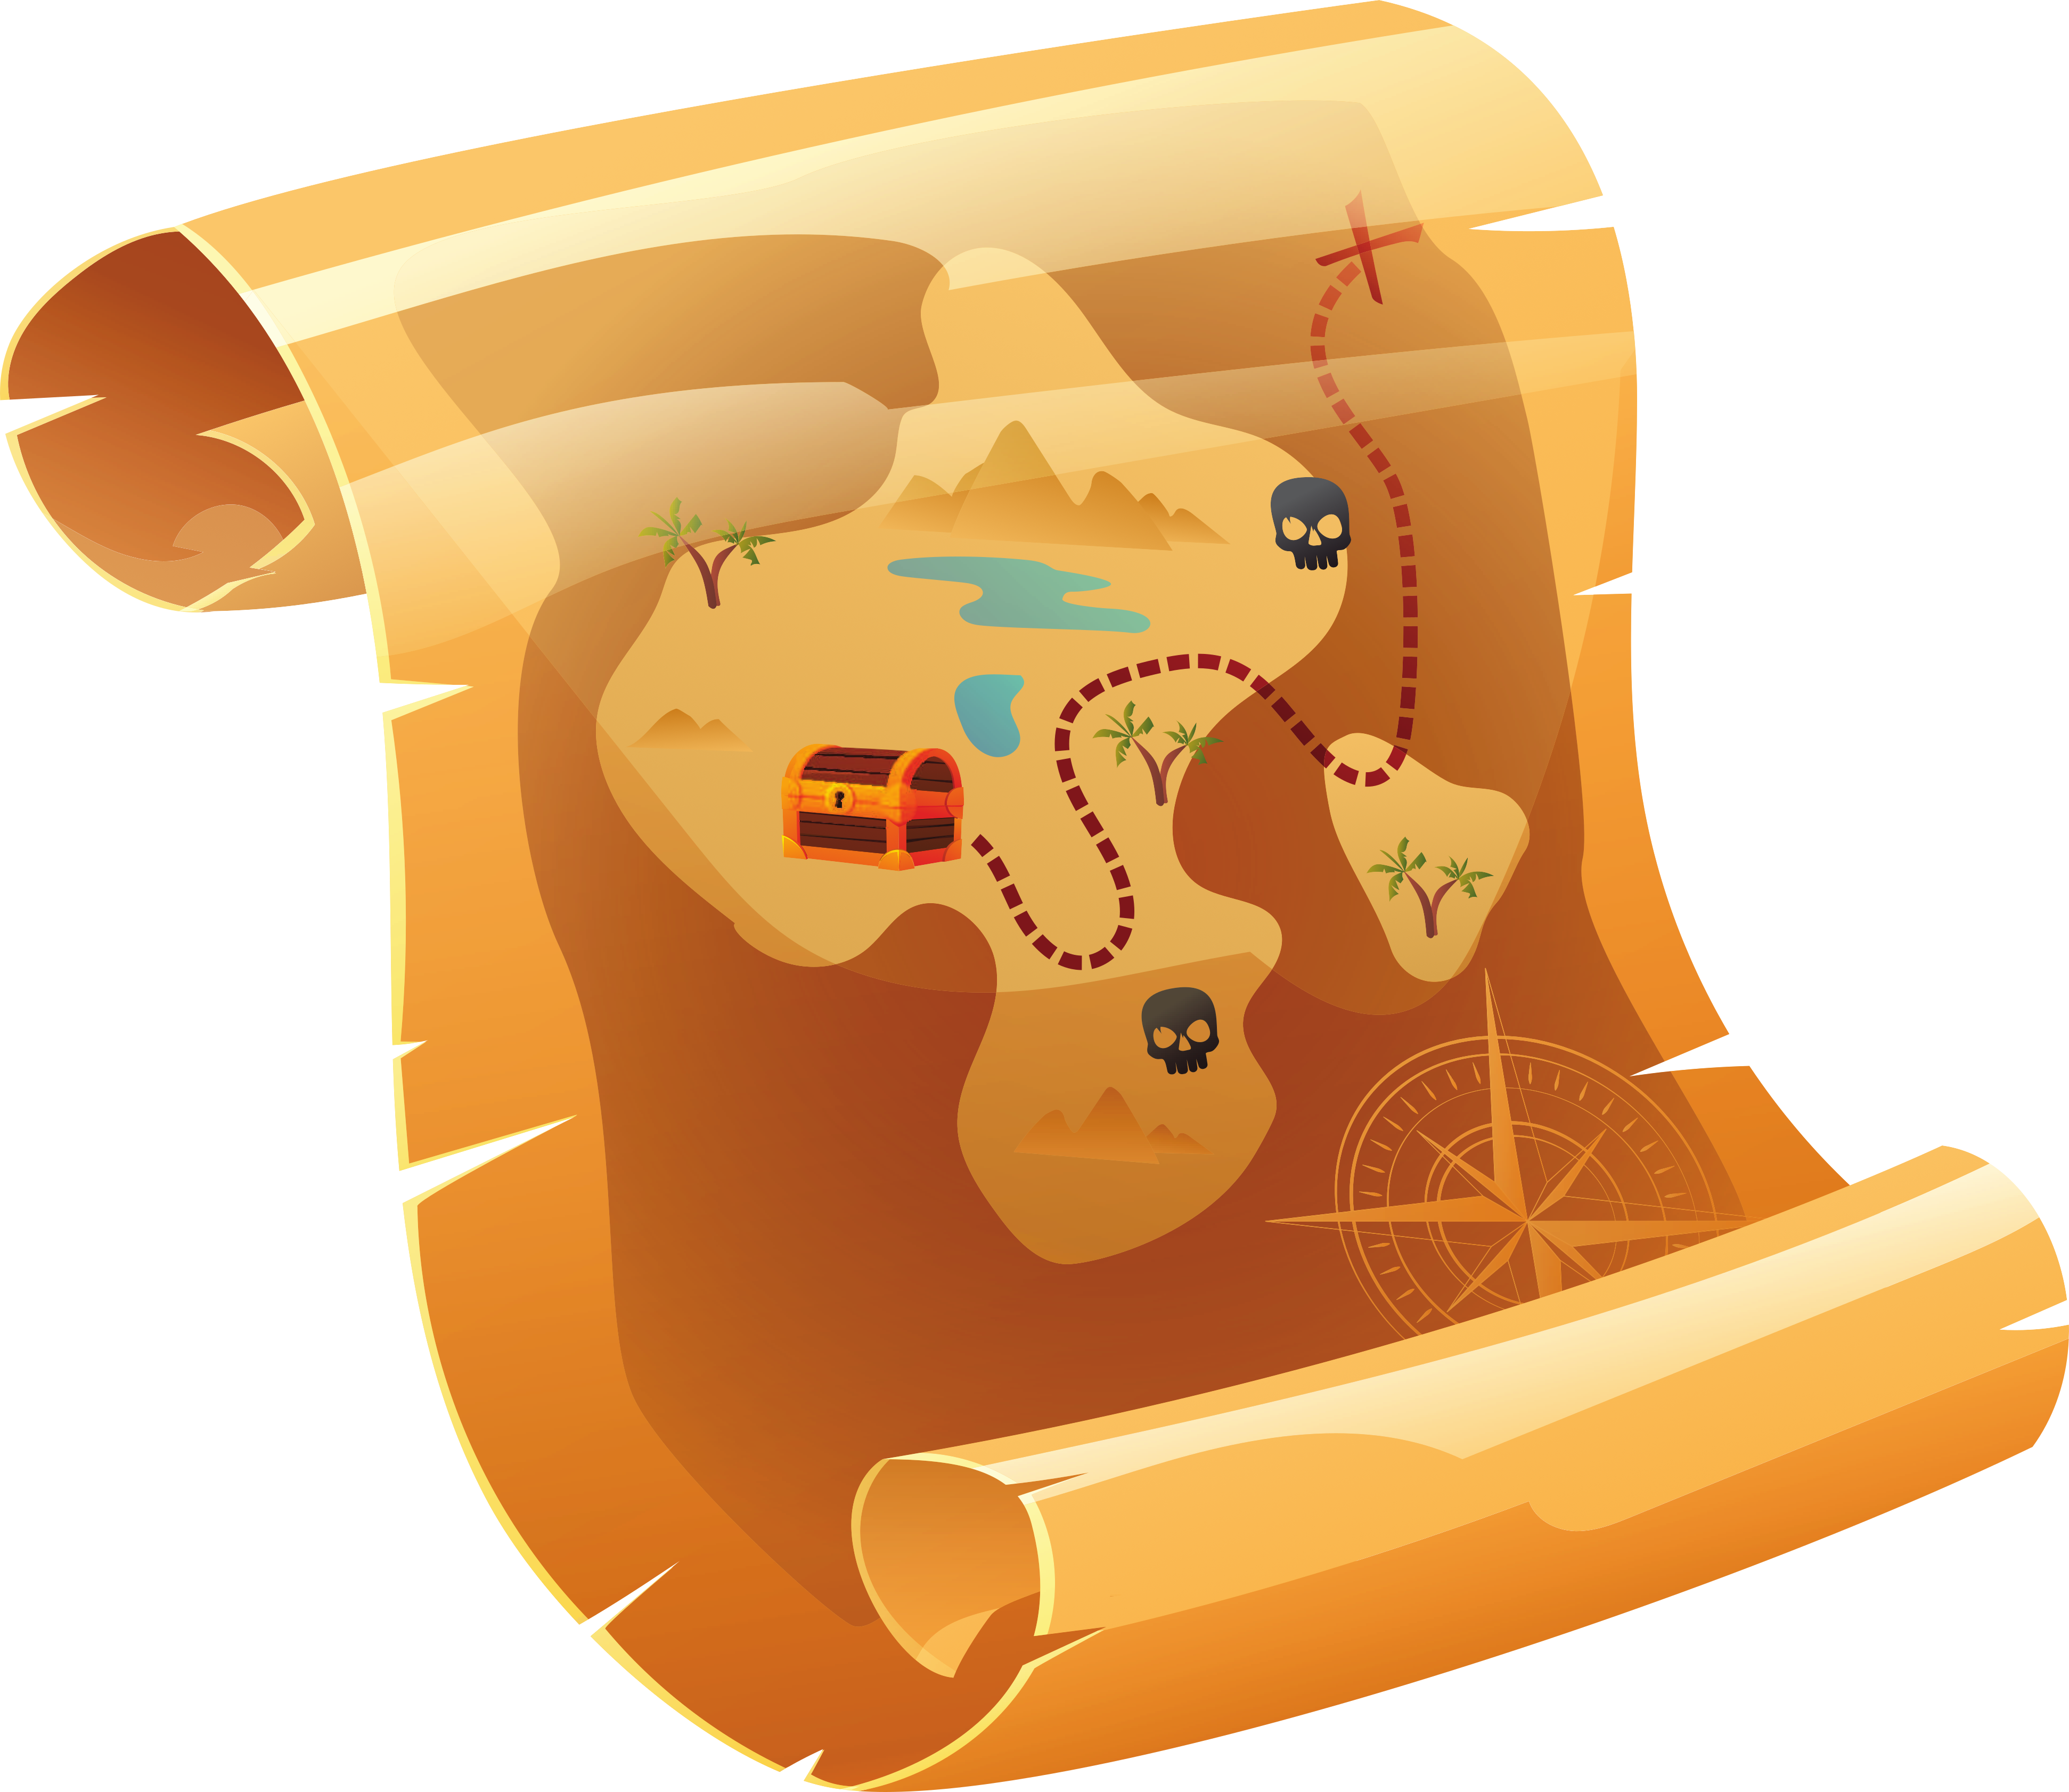
\includegraphics[width=1.0cm]{Images/treasure-map.png}};}
\end{minipage}
\ 
\begin{minipage}{6cm}
\raggedright
\maptext
\end{minipage}

\begin{minipage}{1.5cm}
\tikz{\node[draw, thick, minimum width=1.5cm, minimum height=1.5cm, inner sep=0pt, rounded corners=3mm] at (0,0) {
\includegraphics[height=1.0cm]{Images/compass.png}};}
\end{minipage}
\ 
\begin{minipage}{6cm}
\raggedright
\compasstext
\end{minipage}

\begin{minipage}{1.5cm}
\tikz{\node[draw, thick, minimum width=1.5cm, minimum height=1.5cm, inner sep=0pt, rounded corners=3mm] at (0,0) {
\includegraphics[height=1.0cm]{Images/spyglass.png}};}
\end{minipage}
\ 
\begin{minipage}{6cm}
\raggedright
\spyglasstext
\end{minipage}

\begin{minipage}{1.5cm}
\tikz{\node[draw, thick, minimum width=1.5cm, minimum height=1.5cm, inner sep=0pt, rounded corners=3mm] at (0,0) {
\includegraphics[height=1.0cm]{Images/message-in-a-bottle.png}};}
\end{minipage}
\ 
\begin{minipage}{6cm}
\raggedright
\messagetext
\end{minipage}

\begin{minipage}{1.5cm}
\tikz{\node[draw, thick, minimum width=1.5cm, minimum height=1.5cm, inner sep=0pt, rounded corners=3mm] at (0,0) {
\includegraphics[width=1.0cm]{Images/pistol.png}};}
\end{minipage}
\ 
\begin{minipage}{6cm}
\raggedright
You may discard a pistol at any time to steal one treasure from another character.
\end{minipage}

\begin{minipage}{1.5cm}
\tikz{\node[draw, thick, minimum width=1.5cm, minimum height=1.5cm, inner sep=0pt, rounded corners=3mm] at (0,0) {
\includegraphics[height=1.0cm]{Images/black-spot.png}};}
\end{minipage}
\ 
\begin{minipage}{6cm}
\raggedright
After each round, steal one random treasure from another character. Lose five points if you have the black spot at~the end of the game.
\end{minipage}
